\section{Method}
The architecture of GAR-Font is illustrated in Figure~\ref{fig: Model}. Our framework comprises three core components:

\noindent\textbf{A global-aware tokenizer (G-Tok)} discretizes glyphs into tokens, capturing intricate structure and global visual style.

\noindent\textbf{An AR generator with multimodal style encoder} first learns from visual inputs to establish a stable style space, and then employs a lightweight language-style adapter for multimodal style control.

\noindent\textbf{A post-refinement} enhances structural fidelity and style coherence for high-quality few-shot font generation.

Given a content glyph, a few style references, and optional text, GAR-Font encodes and aggregates content and style, autoregressively generates codebook representations and decodes them softly into high-quality glyphs, which are subsequently improved by a post-refining stage. The details of each module adopted in the proposed GAR-Font will be presented in the following subsections.

\subsection{Global-aware Tokenizer}
The Global-aware Tokenizer (G-Tok), shown in Figure~\ref{fig: G-tok}, encodes glyphs into tokens using a hybrid CNN–ViT encoder, a vector quantizer, and a causal hybrid decoder. By fusing local convolutional features with Transformer-based global context, it captures fine-grained structure and overall style, enabling coherent, high-quality font synthesis.

\vspace{-3mm}
\paragraph{Hybrid encoding.} Given a glyph image $\mathbf{I} \in \mathbb{R}^{H \times W \times 3}$, a CNN encoder $E_{\text{CNN}}$ extracts local stroke features, which are flattened and aggregated through a ViT encoder $E_{\text{ViT}}$:
\begin{equation}
    \mathbf{T} = E_{\text{ViT}}\big(\mathrm{Proj}(E_{\text{CNN}}(\mathbf{I})) + \mathbf{P}_{\text{2D}}\big) \in \mathbb{R}^{N\times d},
\end{equation}
where $\mathbf{P}_{\text{2D}}$ refers to the 2D sinusoidal position embeddings~\cite{ViT}, $N$ and $d$ denote token count and embedding dimension. The convolutional backbone preserves spatial locality, capturing fine stroke geometry, while the ViT’s self-attention aggregates tokens globally to enforce style fidelity. This hybrid design captures both structure fidelity and long-range style dependencies.
\vspace{-4mm}
\paragraph{Vector Quantization.} Following standard VQ-VAE~\cite{VQ_VAE} and VQ-GAN~\cite{VQ_GAN}, we discretize latent tokens by mapping them to the nearest entries in a learnable table. We apply the commitment and embedding regularization with an entropy term to stabilize training and preserve diversity.
\vspace{-4mm}
\paragraph{Causal decoding and optimization.} A causal ViT–CNN decoder reconstructs glyph $\hat{\mathbf{I}}$ from quantized tokens, modeling sequential dependencies while convolutional layers refine local details. Figure~\ref{fig: G-tok}(b) illustrates this structure.

The tokenizer is optimized end-to-end with a weighted combination of reconstruction, perceptual, and vector quantization losses:
\begin{equation}
    \mathcal{L}_{\text{tok}} =
\lambda_{\text{rec}}\mathcal{L}_{\text{rec}} +
\lambda_{\text{per}}\mathcal{L}_{\text{per}} +
\lambda_{\text{vq}}\mathcal{L}_{\text{vq}},
\end{equation}
where $\mathcal{L}_{\text{rec}}=\|\mathbf{I}-\hat{\mathbf{I}}\|_1$ denotes the L1 reconstruction loss, $\mathcal{L}_{\text{per}}=\|\Phi(\mathbf{I})-\Phi(\hat{\mathbf{I}})\|_2^2$ represents the perceptual loss, and $\mathcal{L}_{\text{vq}}$ is the standard vector quantization loss. 

\subsection{AR Generator with Multimodal Style Encoder}
Using G-Tok’s global representations, the AR generator performs conditional sequential prediction. To leverage prior FFG insights (Content-style Aggregator) while avoiding the cost of joint image–text training, GAR-Font adopts a decoupled learning paradigm. The generator, aggregator, and style encoder are first trained on visual inputs to learn a stable representation. Based on this foundation, the visual style encoder is extended into a multimodal one through a lightweight, plug-in language adapter that aligns textual cues with learned visual styles, enabling flexible text-guided generation without disturbing the visual prior.

\subsubsection{Pretraining on Visual Modality}
Visualized in Figure~\ref{fig: Training}(a), to build a stable style–content representation, the AR generator is first trained on visual conditions, following the successful practices of prior FFG methods. This ensures robust modeling of both content structure and stylistic variations across glyphs, providing a solid foundation for subsequent multimodal adaptation.
\vspace{-4mm}
\paragraph{Encoders and Content–style Aggregator.} 
As shown in Figure~\ref{fig: Training}(a), we adopt both CNN architectures on the content encoder and the visual style encoder. The Content-style Aggregator follows the previous design~\cite{Fs_Font, LF_Font}. Given a content glyph and $N_s$ style references, the encoders respectively extract content features $\mathbf{F}_c$ and style features$\{\mathbf{F}_{vis_j}\}^{N_s}_{j=1}$. These features are then fused where content queries attend to fine-grained style cues:
\begin{equation}
\tilde{\mathbf{T}}_{\text{vis}} = \mathrm{Aggregator}\big(\mathbf{F}_c, \{\mathbf{F}_{\text{vis}_j}\}_{j=1}^{N_s}\big).
\end{equation}
The aggregated visual representation $\tilde{\mathbf{T}}_{\text{vis}}$ is concatenated with $\mathbf{F}_c$ to form the conditioning input $\mathbf{T}$.
\vspace{-3mm}
\paragraph{Autoregressive modeling and soft decoding.} Conditioned on $\mathbf{T}$, the Transformer-based generator autoregressively predicts the next token at each timestep, producing logits $\mathbf{L}$ over the codebook $\mathcal{C}$ of G-Tok. Instead of standard discrete hard decoding, we employ a soft projection that maps $\mathbf{L}$ onto the codebook 
$\tilde{\mathbf{Z}} = \mathrm{Softmax}(\mathbf{L}) \cdot \mathcal{C}$.
This continuous mapping not only preserves gradient flow during training, enabling pixel-level supervision, but can also be applied at inference. Using soft projection at inference improves stroke continuity and glyph fidelity by leveraging the full expressive capacity of the codebook, yielding smoother and more accurate glyphs compared with discrete hard decoding.
\vspace{-3mm}
\paragraph{Training objectives.} During this visual-pretraining stage, the aggregator, generator, and style encoder are jointly optimized with a combined token and pixel-level loss:
\begin{equation}
\mathcal{L}_{\text{AR}} = \lambda_{\text{CE}}\mathcal{L}_{\text{CE}} + \lambda_{\text{pixel}}\mathcal{L}_{\text{pixel}},
\end{equation}
where $\mathcal{L}_{\text{CE}}$ is the cross-entropy loss over the target token indices $\mathbf{s}$, and $\mathcal{L}_{\text{pixel}}$ measures the L1 reconstruction error between the generated glyph $\hat{\mathbf{I}}_f$ and ground truth $\mathbf{I}_f$. 

\subsubsection{Multimodal Style Encoder Adaptation}
Visual pretraining forms a stable style–content space but lacks high-level conceptual control. To address this, we introduce a lightweight, plug-in language adapter that aligns textual design cues with visual style representations, as shown in Figure~\ref{fig: Training}(b). Through this adapter, the style encoder is extended into a multimodal form, enabling flexible text-guided modulation without disrupting the visual prior.
\vspace{-3mm}
\paragraph{Vision-language Adapter.} The adapter bridges textual descriptions and visual style features through an iterative cross-attention mechanism. Specifically, a subset of visual style features $\{\mathbf{F}_{vis_j}\}^{k}_{j=1}$ is first extracted from $k<N_s$ reference glyphs by the visual style encoder, while a textual font description embedding is derived from a pretrained Flan-T5 encoder. The text embedding is projected into the visual feature space and iteratively refined by attending to the given style features. The aligned textual–visual token is then spatially expanded into $\mathbf{F}_t$ and concatenated with the visual features:
\begin{equation}
\tilde{\mathbf{F}}_{mm} = [\mathbf{F}_{vis_1}, \ldots, \mathbf{F}_{vis_k}, \mathbf{F}_t].
\end{equation}
\paragraph{Training objectives.} 
The multimodal style encoder may produce features $\tilde{\mathbf{F}}_{mm}$ with token lengths different from those of the visual-only encoder, due to variations in the number of visual references. Thus, we supervise training on their aggregated objectives. Specifically, $\tilde{\mathbf{T}}_{\text{mm}}$ and $\tilde{\mathbf{T}}_{\text{vis}}$ are obtained by aggregating $k$ visual plus one textual reference, and all $N_s$ visual references, respectively. We train the adapter by minimizing the $\ell_2$ distance between these two aggregated representations:
\begin{equation}
\mathcal{L}_{\text{adapt}} = \|\tilde{\mathbf{T}}_{\text{mm}} - \tilde{\mathbf{T}}_{\text{vis}}\|_{2}^{2}.
\end{equation}
\vspace{-1mm}
This objective encourages the multimodal encoder to internalize stylistic intent consistent with the full-visual setting, facilitating effective text–style substitution and reducing reliance on visual inputs.
\begin{figure}[t!]
    \centering
    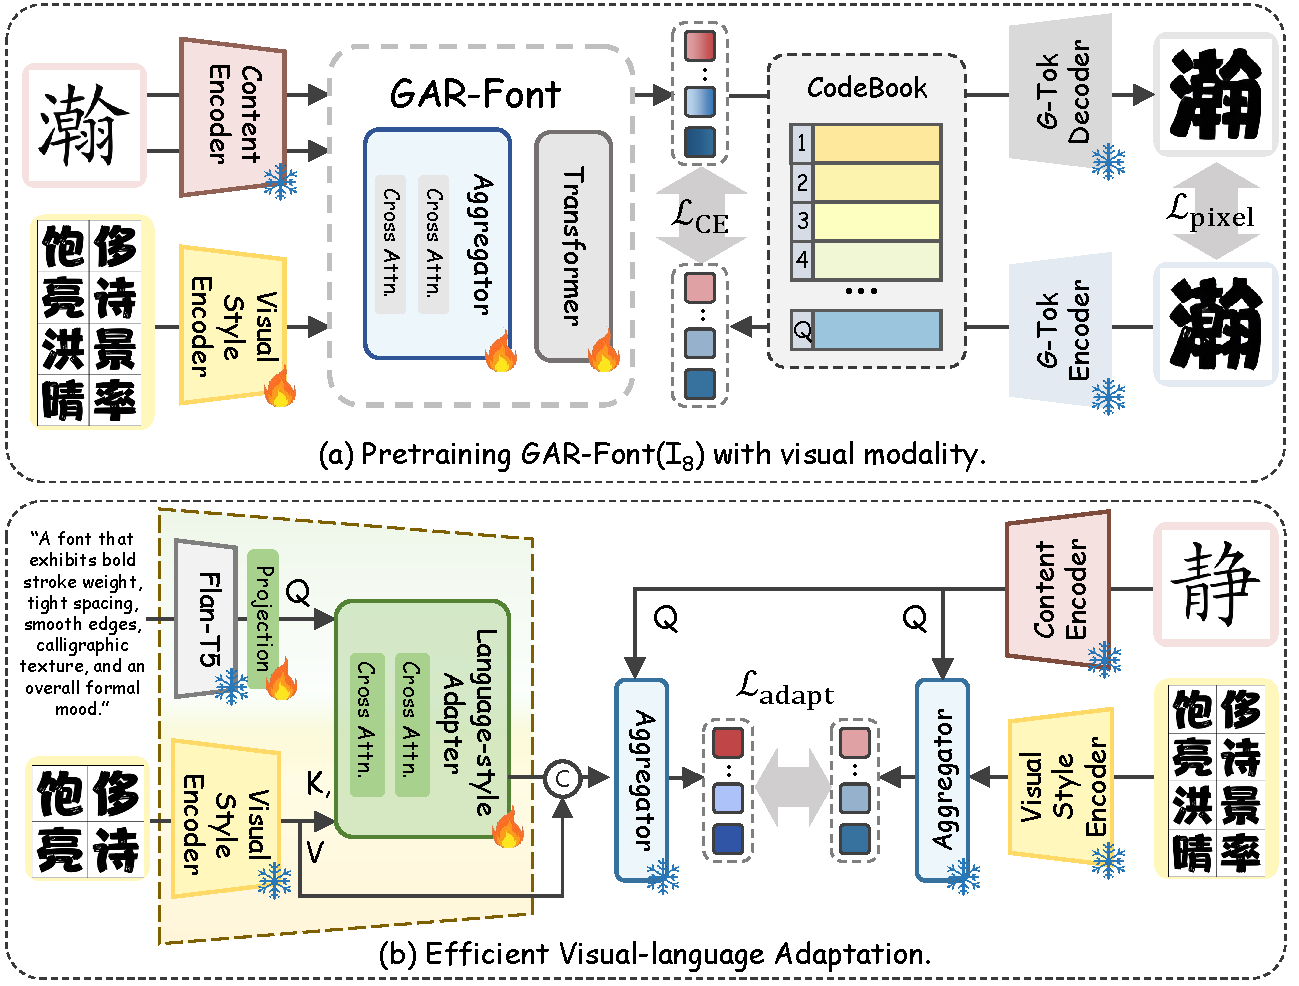
\includegraphics[width=\linewidth]{IMGS/Fig3_Train.pdf}
    \vspace{-5mm}
    \caption{GAR-Font adopts a two-stage training: (a) Visual Pretraining builds a stable content–style space via token and pixel losses; (b) Vision–language Adaptation aligns text embeddings with style features with a lightweight adapter for text-guided generation while preserving visual priors.}
    \label{fig: Training}
    \vspace{-5mm}
\end{figure}
\vspace{-1mm}
\subsection{Post-refinement}
GAR-Font adopts a two-stage post-refinement to improve few-shot style generalization and structural accuracy: novel font adaptation (NFA) and structural enhancement (SE).
\vspace{-3mm}
\paragraph{Novel font adaptation (NFA) for few-shot generalization.} The pretrained generator learns general font patterns but fails to model unseen styles precisely. NFA mitigates this by performing a lightweight adaptation using a few reference glyphs, updating the LoRA layers of the Transformer generator with a mixed token–pixel loss:
\begin{equation}
\mathcal{L}_{\text{SFT}}=\lambda_{\text{CE}}\mathcal{L}_{\text{CE}}+\lambda_{\text{pixel}}\mathcal{L}_{\text{pixel}},
\end{equation}
where $\mathcal{L}_{\text{CE}}$ is the token cross-entropy and $\mathcal{L}_{\text{pixel}}=|\hat{\mathbf{I}}-\mathbf{I}|_1$ encourages pixel-level accuracy. This yields stable few-shot adaptation and better preservation of unseen styles.
\vspace{-3mm}
\paragraph{Structural enhancement (SE) for precise glyph reconstruction.}
While NFA enhances style fidelity, minor structural distortions may remain. To enhance structural clarity and readability, SE further refines glyphs using a group-relative optimization based on GRPO~\cite{DeepseekMath_GRPO}. The generator is treated as a policy $\pi_\theta$ that outputs token sequences $\mathbf{s}$; each decoded glyph receives a composite reward:
\begin{equation}
r=\lambda_{\text{ocr}}\,r_{\text{ocr}}+\lambda_{\text{style}}\,r_{\text{style}},
\end{equation}
\vspace{-1mm}
where $r_{\text{ocr}}$ is obtained from a pretrained OCR model as
\vspace{-2mm}
\begin{equation}
r_{\text{ocr}}=
\begin{cases}
p_{\text{ocr}}, & \text{if } \hat{y}=y,\\[3pt]
0, & \text{otherwise.}
\end{cases}
\end{equation}

Here $p_{\text{ocr}}$ is recognition confidence, and $r_{\text{style}}$ measures consistency with the reference style using a pretrained style discriminator.

%with $p_{\text{ocr}}$ denoting the recognition confidence and $y$ the ground-truth label. $r_{\text{style}}$ evaluates stylistic consistency with reference fonts and mitigates style degradation using a pretrained style discriminator.

Rewards are normalized within each sampled group to compute advantages $A^{(k)} = \frac{r^{(k)} - \mu(r)}{\sigma(r)}$. SE updates only the LoRA layers by maximizing advantage-weighted likelihood with KL regularization to a frozen reference policy:
\vspace{-1mm}
\begin{equation}
\mathcal{L}_{\text{SE}} \!=\! -\mathbb{E}_{\mathbf{s}\sim\pi_\theta}\big[A(\mathbf{s})\log\pi_\theta(\mathbf{s})\big]+\beta\,\mathrm{KL}(\pi_\theta\|\pi_{\text{ref}}),
\end{equation}
where $A(\mathbf{s})$ denotes the group-normalized advantage and $\pi_{\text{ref}}$ is the frozen reference policy used for stability.  

% % The architecture of GAR-Font is illustrated in Figure~\ref{}.
% % Our training pipeline comprises three stages.
% % First, a Global-aware Tokenizer based on a hybrid CNN–ViT design discretizes glyphs into compact tokens that encode both local stroke details and global stylistic dependencies.
% % Second, an Autoregressive Generator conditioned on content and style references models target glyph tokens via a Transformer decoder, ensuring structural integrity and stylistic coherence.
% % Finally, a Post-Training Refinement stage combining supervised fine-tuning and GRPO-based reinforcement learning further enhances generalization and structural fidelity.
% % This unified design enables multimodal, text-driven, few-shot font generation with consistent global style. \lyx{SHOULD MODIFY DEPENDS ON THE VISUALIZATION! NOW WE DON'T HAVE A THREE-STAGE VISUAL!!!!!!}

% The architecture of GAR-Font is illustrated in Figrue ~\ref{}.
% Our framework comprises two sequential training stages and one auxiliary module for multimodal guidance. 

% In the pre-training stage, a global-aware tokenizer is trained to discretize glyphs into compact visual tokens, which are then modeled by an autoregressive generator to reconstruct target glyphs with coherent structure and style.

% On top of the pretrained generator, a lightweight language-style adapter injects textual stylistic cues into the visual embedding space, enabling multimodal control and improving generation quality under limited reference conditions.

% Finally, the post-training stage combines supervised fine-tuning and GRPO-based reinforcement learning to further improve structural fidelity and generalization on novel fonts.


% \subsection{Global-aware Tokenizer}

% The Global-Aware Tokenizer (G-Tok) discretizes glyphs into compact tokens encoding both structural and stylistic information. It consists of a hybrid CNN–ViT encoder, a vector quantizer, and a causal hybrid decoder.
% \begin{figure*}
% \centering
% \includegraphics[width=1.0\linewidth]{TEMP_IMGS/TEMP_G_Tok.jpg}
% \end{figure*}

% \paragraph{Hybrid encoding.} Given a glyph image $\mathbf{I} \in \mathbb{R}^{H \times W \times 3}$, a CNN encoder $E_{\text{CNN}}$ extracts local stroke features, which are flattened and aggregated through a ViT encoder $E_{\text{ViT}}$:
% \begin{equation}
%     \mathbf{T} = E_{\text{ViT}}\big(\mathrm{Proj}(E_{\text{CNN}}(\mathbf{I})) + \mathbf{P}_{\text{2D}}\big) \in \mathbb{R}^{N\times d},
% \end{equation}
% where $\mathbf{P}_{\text{2D}}$ denotes 2D sinusoidal positional embeddings~\cite{ViT}, $N$ and $d$ denote token count and embedding dimension. The convolutional backbone ensures strong spatial locality, critical for capturing the fine-grained stroke geometry. At the same time, multi-head self-attention in the ViT encoder enhances global style consistency by aggregating token information across all spatial positions. This hybrid design captures both structure fidelity and long-range style dependencies crucial for font synthesis.

% \paragraph{Vector Quantization.} We adopt a standard vector quantization scheme following VQ-VAE~\cite{VQ_VAE} and VQ-GAN~\cite{VQ_GAN}, where latent tokens are discretized by mapping to the nearest entries in a learnable codebook. To stabilize codebook usage and preserve representational diversity, we employ commitment and embedding regularization with an additional entropy term. The resulting discrete sequence serves as the autoregressive modeling target.

% \paragraph{Causal decoding and optimization.} A causal ViT-CNN decoder reconstructs glyphs from quantized tokens, integrating global self-attention with local convolutional refinement. 
% The tokenizer is optimized end-to-end with a weighted combination of reconstruction, perceptual, and vector quantization losses:
% \begin{equation}
%     \mathcal{L}_{\text{tok}} =
% \lambda_{\text{rec}}\mathcal{L}_{\text{rec}} +
% \lambda_{\text{per}}\mathcal{L}_{\text{per}} +
% \lambda_{\text{vq}}\mathcal{L}_{\text{vq}},
% \end{equation}
% where $\mathcal{L}_{\text{rec}}=\|\mathbf{I}-\hat{\mathbf{I}}\|_1$ denotes the L1 reconstruction loss, $\mathcal{L}_{\text{per}}=\|\Phi(\mathbf{I})-\Phi(\hat{\mathbf{I}})\|_2^2$ represents the perceptual loss, and $\mathcal{L}_{\text{vq}}$ is the standard vector quantization loss. 
% This training yields discrete representations that preserve both structural fidelity and global stylistic coherence for downstream autoregressive generation.
% \lyx{PLEASE DESIGNATE ALL THE EQUATIONS, WHETHER THEY ARE WRITTEN CORRECTLY AND WHETHER THEY HAVE ALL THE COMPONENTS WELL-DEFINED (e.g, where A denotes xxx, B denotes xxx,  etc.). PLEASE BE SURE ALL THE COMPONENTS ARE DEFINED!!!!}



% \subsection{Autoregressive Generator}
% The autoregressive generator produces target glyphs that preserve the structural layout of a content glyph $\mathbf{I}_c$ while adopting styles from $N_s$ reference glyphs $\{\mathbf{I}_{s_j}\}_{j=1}^{N_s}$. The generation pipeline consists of three stages: content–style encoding and fusion, autoregressive token prediction, and image reconstruction from predicted tokens (Fig.~\ref{}).

% \begin{figure}[t]
%   \centering
%   %\fbox{\rule{0pt}{2in} \rule{0.9\linewidth}{0pt}}
%   \includegraphics[width=1.0\linewidth]{TEMP_IMGS/TEMP_Generator_2.jpg}

%    \caption{EXAMPLE2 : Architecture of GAR-Font}
%    \label{fig:onecol}
% \end{figure}

% \paragraph{Content-style encoding and fusion.} A content encoder $E_c$ and a style encoder $E_s$ extract features from the content and style glyphs, respectively. Iterative cross-attention blocks~\cite{Fs_Font, VQ_Font} inject fine-grained style information into content features, and the resulting style-enhanced features are concatenated with the content features to form the final conditioning representation $\mathbf{T}_{\text{cond}}$ (as illustrated in Figure~\ref{}).

% \paragraph{Autoregressive token generation.} The Transformer-based autoregressive generator takes $\mathbf{T}_{cond}$ as context and models the sequential dependencies within the discrete token sequence $\mathbf{s}$ generated by G-Tok. Predicted logits $\mathbf{L}$ are softly projected onto the codebook $\mathcal{C}$ as $\tilde{\mathbf{Z}}=\mathrm{Softmax}(\mathbf{L})\mathcal{C}$, producing continuous embeddings that are decoded by the G-Tok decoder $D$ to reconstruct the glyph image $\hat{\mathbf{I}}_f$. This differentiable decoding maintains gradient flow and enables smoother transitions in the latent space, bridging the gap between discrete token prediction and continuous image reconstruction to enhance visual quality.

% \paragraph{Training objectives.} The generator is optimized with a combined token and pixel-level loss:

% \begin{equation}
% \mathcal{L}_{\text{total}} = \lambda_{\text{CE}}\mathcal{L}_{\text{CE}} + \lambda_{\text{pixel}}\mathcal{L}_{\text{pixel}},
% \end{equation}
% where $\mathcal{L}_{\text{CE}}$ is the cross-entropy loss over the target token indices $\mathbf{s}$, and $\mathcal{L}_{\text{pixel}}$ measures L1 reconstruction error between the generated glyph $\hat{\mathbf{I}}_f$ and ground truth $\mathbf{I}_f$. This compact objective enforces accurate sequential modeling and high-fidelity glyph reconstruction.
% \lyx{YOU MAY ADD MORE DETAILS, AND ALSO THE DETAILS OF MULTIMODALITY!!!!!!}



% \subsection{Lightweight Language-Style Adapter}
% To enhance few-shot generation under more limited reference conditions, we propose a lightweight language-style adapter that injects textual stylistic guidance into the pretrained autoregressive generator without additional multimodal pretraining. The adapter establishes a shared representation space between textual font descriptions and visual style embeddings, enabling flexible multimodal control.

% \paragraph{Language–style feature alignment.}
% Given a subset of visual style features ${\mathbf{F}_{s_j}},{j=1,2,..,k}$ extracted from $k<N_s$ style reference glyphs  through the style encoder $E_s$ and a textual font description embedding $\mathbf{E}_t$ obtained from a pretrained T5 encoder, the adapter aligns these modalities through iterative cross-attention interactions.
% Specifically, the text embedding $\mathbf{E}_t$ is first projected into the visual feature space and then refined by attending to stylistic visual features ${\mathbf{F}_{s_j}},{j=1,2,..,k}$, allowing the text representation to absorb fine-grained visual attributes from limited references. This process effectively injects stylistic semantics into the textual embedding while maintaining its global descriptive coherence.

% \paragraph{Language-style Fusion and pseudo-style representation.}
% After alignment, the aggregated textual-visual token is expanded spatially and concatenated with the remaining visual style features to form a unified pseudo-style representation:
% \begin{equation}
% \tilde{\mathbf{F}}_s = [\mathbf{F}_{s_1}, \ldots, \mathbf{F}_{s_k}, \mathbf{F}_t],
% \end{equation}
% where $\mathbf{F}_t$ denotes the text-fused representations. This fused style representation is then integrated with the content encoding through the generator’s feature fusion module, serving as a multimodal conditioning input for subsequent autoregressive generation.

% \paragraph{Training objectives.}
% The adapter is optimized under a teacher–student framework, where a pretrained generator serves as the teacher to provide full style fusion supervision. The teacher produces complete fused feature representations using all available style references, while the student—equipped with the proposed adapter—predicts pseudo-style representations from fewer visual references and corresponding textual descriptions.
% By minimizing the discrepancy between teacher and student fused representations, the adapter learns to recover missing stylistic cues from linguistic guidance and to generalize across unseen font styles.
% The overall training objective is defined as:
% \begin{equation}
% \mathcal{L}_{\text{adapter}} = \|\tilde{\mathbf{F}}_{s}^{\text{student}} - \tilde{\mathbf{F}}_{s}^{\text{teacher}}\|_{2}^{2},
% \end{equation}
% where $\tilde{\mathbf{F}}_{s}^{\text{teacher}}$ and $\tilde{\mathbf{F}}_{s}^{\text{student}}$ denote the fully fused and pseudo-style fused feature representations, respectively.

% This feature-level reconstruction loss enforces consistent multimodal alignment and encourages the adapter to infer complementary visual information from textual style descriptions and limited references.


% \subsection{}

% \subsection{Post-training}
% To improve stylistic fidelity and glyph structure, GAR-Font applies a two-stage post-training: supervised fine-tuning (SFT) for few-shot adaptation and reinforcement learning (RL) for structural refinement.

% \paragraph{Supervised fine-tuning (SFT) for novel font adaptation.}
% While the pretrained generator captures overall font styles, it still tends to overfit seen styles when adapting to unseen ones, reducing style fidelity. To mitigate this, GAR-Font applies a supervised fine-tuning (SFT) stage for targeted adaptation using a few reference glyphs. 
% SFT updates a small subset of parameters (style encoder, fusion module, and LoRA layers) and optimizes a combined token–pixel objective:
% \begin{equation}
% \mathcal{L}_{\text{SFT}}=\lambda_{\text{CE}}\mathcal{L}_{\text{CE}}+\lambda_{\text{pixel}}\mathcal{L}_{\text{pixel}},
% \end{equation}
% where $\mathcal{L}_{\text{CE}}$ denotes the cross-entropy over target token indices and $\mathcal{L}_{\text{pixel}}=\|\hat{\mathbf{I}}-\mathbf{I}_{\text{tar}}\|_1$ measures L1 reconstruction between the decoded glyph $\hat{\mathbf{I}}$ and ground truth $\mathbf{I}_{\text{tar}}$. 
% This lightweight SFT ensures stable few-shot adaptation, enabling faithful preservation of unseen styles while maintaining content consistency.

% \paragraph{Reinforcement learning for glyph structural refinement.}
% While SFT improves style fidelity, generated glyphs may still exhibit subtle structural distortions. To enhance structural clarity and readability, we introduce a reinforcement learning (RL) stage built upon the Group Relative Policy Optimization (GRPO) framework~\cite{DeepseekMath_GRPO}. The generator is fine-tuned as a policy $\pi_\theta$ that produces token sequences $\mathbf{s}$ conditioned on $\mathbf{T}_{cond}$. Each generated glyph $\hat{\mathbf{I}}$ receives a composite reward:
% \begin{equation}
% r=\lambda_{\text{ocr}}\,r_{\text{ocr}}+\lambda_{\text{style}}\,r_{\text{style}},
% \end{equation}
% where $r_{\text{ocr}}$ is derived from an OCR recognizer as
% \begin{equation}
% r_{\text{ocr}}=
% \begin{cases}
% p_{\text{ocr}}, & \text{if } \hat{y}=y,\\[3pt]
% 0, & \text{otherwise,}
% \end{cases}
% \end{equation}
% with $p_{\text{ocr}}$ denoting the recognition confidence and $y$ the ground-truth label, while $r_{\text{style}}$ measures stylistic consistency to the references and prevents collapse via a pretrained style discriminator.

% We normalize rewards across the sampled group and compute group-relative advantages $A^{(k)} = \frac{r^{(k)} - \mu(r)}{\sigma(r)}$. The policy is updated by maximizing the advantage-weighted log-likelihood with a KL regularizer to a frozen reference policy:
% \begin{equation}
% \mathcal{L}_{\text{GRPO}} \!=\! -\mathbb{E}_{\mathbf{s}\sim\pi_\theta}\big[A(\mathbf{s})\log\pi_\theta(\mathbf{s})\big]+\beta\,\mathrm{KL}(\pi_\theta\|\pi_{\text{ref}}),
% \end{equation}
% where $A(\mathbf{s})$ denotes the group-normalized advantage and $\pi_{\text{ref}}$ is the frozen reference policy used for stability.  
% .


% %\subsection{Global-aware Tokenizer}
% %The global-aware hybrid CNN-ViT tokenizer (G-Tok) constitutes the foundational representation module of GAR-Font, providing discrete, structural and stylistic context-rich representations for autoregressive modeling. As illustrated in <<Fig>>, our tokenizer consists of three major parts : a hybrid CNN-ViT Encoder, Vector Quantizer, and hybrid ViT-CNN Decoder. By combining the spatial sensitivity of convolutions with the global contextual modeling of Transformers, the tokenizer achieves superior extraction of both structural details and holistic stylistic features, which are essential for the FFG task.

% %\subsubsection{Local-Global Hybrid Encoding for Glyph Representation.}
% %Given an input glyph image $\mathbf{I}_f \in \mathbb{R}^{H \times W \times 3}$, the encoder first extracts spatially coherent patch-level features through a series of convolutional blocks:

% %$$\mathbf{F}_{e-cnn} = E_{cnn}(\mathbf{I}_f) \in \mathbb{R}^{C \times h \times w}$$

% %The convolutional backbone ensures strong spatial locality and structural precision, which are critical for capturing the intricate compositional patterns of glyphs.

% %To enhance global perception, $\mathbf{F}_{\text{cnn}}$ is projected into a latent embedding space and flattened into a token sequence for subsequent contextual aggregation:

% %$$\mathbf{T}_{e-cnn} = \mathrm{Flatten}(\mathrm{Proj}(\mathbf{F}_{e-cnn})) \in \mathbb{R}^{N \times d}, \quad N = h \times w$$


% %These tokens are then fed into a Vision Transformer encoder $E_{\text{ViT}}$, equipped with 2D positional embeddings:

% %$$\mathbf{T}_{e-vit} = E_{vit}(\mathbf{T}_{e-cnn} + \mathbf{P}_{2D}) \in \mathbb{R}^{N \times d}, \quad N = h \times w$$

% %Through multi-head self-attention, each token aggregates information across all spatial positions an gains larger receptive fields, enabling the model to capture long-range dependencies and global stylistic coherence.

% %By unifying convolutional local feature extraction capability and transformer-based  global context modeling power, our encoder generates structural precise and globally contextualized representations.


% %\subsubsection{Vector Quantization and Token Discretization.}
% %Folowing the principles of VQ-VAE ~\cite{VQ_VAE} and VQ-GAN ~\cite{VQ_GAN} , the continuous latent embeddings produced by the encoder are discretized into a learnable codebook, denoted as $ C = \{c_{k} \in R^{d}\}^{K}_{k=1}$. 
% %After encoding a glyph image into continuous tokens $\mathbf{T}_{vit} \in \mathbb{R}^{N \times d}$, token-wise quantization $q(\text{·})$ is performed to replace each embedding with its nearest entry in the codebook : 

% %$$\mathbf{Z}_q(i) = q(\mathbf{T}_{e-vit}(i)) := \arg\min_{\mathbf{c}_k \in \mathcal{C}} 
% %\| \mathbf{T}_{e-vit}(i) - \mathbf{c}_k \|_2$$

% %This process yields  a quantized latent representation $Z_{q} \in \mathbb{R}^{N \times d}$ and its corresponding discrete index sequence $s = \{ s_{i}\}^{N}_{i=1}$, which serves as the autoregressive modeling target in subsequent stages.

% %To guide codebook training and encourage diverse codebook usage, we apply the standard vector quantization loss:

% %$$\mathcal{L}_{vq} = \alpha \| sg(T_{e-vit})-Z_{q}\|_{2}^{2}+\beta \| T_{e-vit}-sg(Z_{q})\|_{2}^{2}+\gamma \mathcal{L}_{entropy}$$

% %where $sg(\text{·})$ denotes the stop-gradient operation and $\mathcal{L}_{entropy}$ regularizes codebook utilization entropy to prevent codebook collapse.

% %This discretization process transforms the continuous representation into compact, semantically meaningful discrete tokens, forming the foundation for autoregressive glyph modeling.

% %\subsubsection{Causal Decoding and Reconstruction Objectives.}
% %To reconstruct glyph images from quantized tokens, a causal hybrid ViT-CNN decoder is introduced, mirroring the encoder design while introducing a causal self-attention mechanism. This design models sequential dependencies among tokens, aligned with the autoregressive paradigm of downstream generation process.

% %Given the quantized sequential tokens $\mathbf{Z}_q \in \mathbb{R}^{N \times d}$, 
% %the causal ViT decoder first processes them with 2D positional embeddings:

% %$$ \mathbf{T}_{d-vit} = \text{CausalViT}(\mathbf{Z}_q + \mathbf{P}_{2D}) $$

% %Then, $\mathbf{T}_{d-vit}$ is projected to the latent space and reshaped into a spatial representation:

% %$$ \mathbf{F}_{d-vit} = \text{Reshape}(\text{Proj}(\mathbf{T}_{d-vit})) \in \mathbb{R}^{C \times H \times W} $$

% %which is subsequently decoded by the CNN decoder $D_{cnn}$ to reconstruct the input glyph image:
% %$$ \hat{\mathbf{I}}_f = D_{cnn}(\mathbf{F}_{d-vit}) $$

% %The tokenizer is jointly optimized in an end-to-end manner with a  weighted combination of 
% %reconstruction loss $\mathcal{L}_{rec}$, 
% %perceptual loss $\mathcal{L}_{per}$, 
% %and vector quantization loss $\mathcal{L}_{vq}$:

% %$$ \mathcal{L}_{tokenizer} =\lambda_{rec} \mathcal{L}_{rec} + \lambda_{per}\mathcal{L}_{per} + \lambda_{vq}\mathcal{L}_{vq} $$
% %where $\mathcal{L}_{rec} = \| \mathbf{I}_f - \hat{\mathbf{I}}_f \|_1$ 
% %and $\mathcal{L}_{per} = 
% %\| \Phi(\mathbf{I}_f) - \Phi(\hat{\mathbf{I}}_f) \|_2^2$, 
% %with $\Phi(\cdot)$ denoting a pretrained VGG-based <CITE : VGG ref> perceptual feature extractor.

% %\subsection{Autoregressive Generator}
% %The autoregressive generator synthesizes a target glyph image that preserves the structural layout of a standard content glyph $\mathbf{I}_c \in \mathbb{R}^{H \times W \times 3}$ while maintaining the stylistic patterns from $N_{s}$ style reference glyphs $\{I_{s_{j}}\}^{N_s}_{j=1}$. The process consists of three main stages:(1) content-style encoding with attention-based fusion, (2) autoregressive next-token prediction; and (3) optimization via a weighted combination of token loss and pixel loss. The overall architecture is depicted in <Fig>.

% %\subsubsection{Content–Style Encoding and Fusion.}
% %Following prior FFG works ~\cite{Fs_Font, VQ_Font}, GAR-Font employs a iterative cross-attention mechanism to attentively capture and integrate fine-grained styles. Specifically, a content encoder $E_c$ and a style encoder $E_s$ extract representations $f_{c} \in \mathbb{R}^{hw \times C}$and $f_{s} \in \mathbb{R}^{khw \times C}$ from content glyph $\mathbf{I}_c$ and style glyphs $\{I_{s_{j}}\}^{N_s}_{j=1}$ respectively. A multi-layer Feature Fusion Module (FFM) integrates fine-grained style information through iterative cross-attention:

% %$$ A_{style} = \frac{(W^{Q}f_{c})(W^{K}f_{s})^T}{\sqrt{C}}, f_{cs} = Softmax(A_{style}) \times (W_{V}F_{s})$$

% %where $W^{Q}$, $W^{K}$, $W^{V}$ are learnable parameters to project the extracted features into query and key, and $C$ is the dimension of the key.

% %Stacking $L$ cross-attention blocks progressively results in a completive integration of content and style attributes $F_{fused} \in \mathbb{R}^{hw \times C}$. To maintain structural features, following ~\cite{Fs_Font}, $f_c$ and $F_{fused}$ are concatenated to form the conditioning representation $T_{cond} \in \mathbb{R}^{hw \times 2C}$.

% %\subsubsection{Autoregressive Token Generation.}
% %Conditioned on $T_{cond}$, a Transformer-based autoregressive generator models the sequential dependencies among discrete token indices $ s = \{s_{i}\}_{i=1}^{N}$ corresponding to the quantized embeddings from G-Tok.

% %Formally, the autoregressive model defines a joint distribution over tokens as :

% %$$ P(\mathbf{s} \,|\, \mathbf{T}_{cond}) = \prod_{i=1}^{N} P(s_i \,|\, s_{<i}, \mathbf{T}_{cond})$$

% %This causally sequential formulation aligns with the tokenization stage, modeling the long-range structural dependencies and stylistic coherence.

% %The autoregressively predicted logits $\mathbb{L} $ are softly quantized via the the G-Tok codebook $\mathcal{C}$:
% %$$ \tilde{\mathbf{Z}} = \mathrm{Softmax}(\mathbf{L}) \, \mathcal{C} $$.

% %The resulting continuous embeddings $\tilde{\mathbf{Z}}$ are directly fed into the G-Tok decoder $D$, which integrates global contextual reasoning from the ViT layers and spatial detail restoration form the CNN backbone to reconstruct the target glyph image :

% %$$\hat{\mathbf{I}}_{f} = D(\tilde{\mathbf{Z}})$$


% %This differentiable decoding strategy preserves gradient flow and stabilizes training process, which is critical for high-fidelity font synthesis.

% %\subsubsection{Training Objectives.}
% %The autoregressive generator is optimized with two objectives : a token-level prediction loss and a pixel-level reconstruction loss.

% %The token-level prediction loss enforces accurate sequential modeling by guiding the generator to predict each target token conditioned on preceding tokens and $T_{cond}$. It is formulated as a standard corss-entropy loss over the ground-truth token indices $mathbf{s}$ the predicted logits $\mathbf{L}$ :

% %$$\mathcal{L}_{\text{CE}} = - \frac{1}{N} \sum_{i=1}^{N} \log P(s_i \,|\, s_{<i}, \mathbf{T}_{cond}) $$,

% %where $\mathbf{T}_{cond}$ represents the fused conditioning features and $N$ is the token sequence length.

% %To further enhance the perceptual and structural quality of the reconstructed glyphs, the predicted logits $\mathbf{L}$ are softly quantized via G-Tok codebook $\mathcal{C}$, producing continuous token embeddings that are decoded by G-Tok decoder $D$ to yield the reconstructed glyph $\hat{\mathbf{I}}_f$. The reconstruction loss measures pixel-level fidelity between the generated glyph and the ground truth:
% %$$ \mathcal{L}_{\text{pixel}} = \| \hat{\mathbf{I}}_{f} - \mathbf{I}_{f} \|_1 $$

% %The final training objective combines the two loss : 

% %$$\mathcal{L}_{\text{total}} = \lambda_{\text{CE}} \mathcal{L}_{\text{CE}} + \lambda_{\text{pixel}} \mathcal{L}_{\text{pixel}}.$$



% %\subsection{Post Training}
% %To further refine stylistic features and structural precision, GAR-Font first introduces a post-training stage composed of supervised fine-tuning (SFT) and reinforcement learning (RL). The SFT phase enhances few-shot adaptability and stylistic stability, while the RL phase strengthens structural coherence and readability of generated glyphs.

% %\subsubsection{Supervised Fine-tuning for Novel Fonts Adaptation}
% %Although our pretrained generator effectively captures holistic font style representations, it still faces the same challenge as existing few-shot font generation(FFG) methods when adapting to unseen fonts-tending to approximate novel styles by simply aligning them with a similar seen ones, which compromises style fidelity. To mitigate this bias, GAR-Font performs a supervised fine-tuning (SFT) stage that achieves targeted Adaptation to new fonts with only a few reference glyphs.

% %The procedure follows the same training pipeline as pretraining, while updates only a small set of parameters, including those in the style encoder, feature fusion module, and the LoRA-adapted layers of the autoregressive generator.

% %Given a target glyph image $I_{tar}$, its content glyph $I_c$ and a set of style references $\{I_{s_{j}}\}$, the generator predicts discrete tokens and reconstructs the glyph under two training objectives:

% %$$\mathcal{L}_{CE} = \text{CrossEntropy}(\text{logits}, \text{targets}),\mathcal{L}_{pixel} = \| \hat{\mathbf{I}} - \mathbf{I}_{tar} \|_{1}$$

% %The total supervised fine-tuning loss is:

% %$$ \mathcal{L}_{total} = \lambda_{CE} \mathcal{L}_{CE} + \lambda_{pixel} \mathcal{L}_{pixel}
% % $$

% %This SFT process ensures stable few-shot adpation, enabling GAR-Font to faithfully preserve stylistic cues from unseen fonts while maintaining high content consistency.


% %\subsubsection{Reinforcement learning for glyph structural refinement}
% %While the SFT stage enhances style fidelity for novel fonts, the generated glyphs may still exhibit subtle structural distortions issues. To further refine the glyph quality, we introduce a reinforcement learning (RL) stage built upon the Group Relative Policy Optimization (GRPO) framework ~\cite{DeepseekMath_GRPO}. The generator is regarded as a policy network $\pi_{\theta}$, which models a probability distribution over token sequences conditioned on the content-style fusion representation $T_{cond}$:

% %$$P_{\theta}(\mathbf{s} \,|\, \mathbf{T}_{cond}) = 
% %\prod_{i=1}^{N} P_{\theta}(s_i \,|\, s_{<i}, \mathbf{T}_{cond})$$

% %At each iteration, multiple candidate token sequences $s^{(k)} ~ \pi_{\theta}(\text{·} | T_{cond})$ are sampled and decoded by the G-Tok decoder $D$ into glyph images  $\hat{\mathbf{I}}^{(k)} = D(q^{-1}(s^{(k)}))$. 

% %To guide the model to generate structurally accurate and clearly readable glyphs, we define a reward function that integrates content accuracy and style consistency. The OCR-based reward $r_{ocr}$ is derived from an external recogintion model (EasyOCR), which predicts the recognized character $\hat{y}$ and confidence score $p_{ocr}$ given the generated glyph $\hat{\mathbf{I}}$ :
% %$$
% %r_{\text{ocr}} =
% %\begin{cases}
% %p_{\text{ocr}}, & \text{if } \hat{y} = y, \\[4pt]
% %0, & \text{otherwise.}
% %\end{cases}
% %$$,
% %where $y$ denotes the ground-truth character label of $\hat{\mathbf{I}}$.

% %In parallel, a style-consistency reward $r_{style}$ is computed using a pretrained style discriminator to prevent style collapse and ensure that stylistic attributes remain faithful to the reference style. 


% %The overall reward is formulated as :

% %$$r = \lambda_{\text{ocr}} r_{\text{ocr}} + \lambda_{\text{style}} r_{\text{style}}$$

% %where $\lambda_{ocr} \gg \lambda_{style} $, since content accuracy is the primary optimization goal.

% %Following GRPO paradigm, rewards across multiple rollouts are normalized to compute the group-relative advantage:

% %$$A^{(k)} = \frac{r^{(k)} - \mu(r)}{\sigma(r)}$$

% %The generator is updated to maximize the advantage-weighted log-likelihood of sampled token sequences, while constrained by a frozen reference policy $\pi_{ref}$ via a KL-regularization term :

% %$$ \mathcal {L}_{\text{GRPO}} =
% %- \mathbb{E}_{\mathbf{s} \sim \pi_{\theta}}
% %\big[ A(\mathbf{s}) \log \pi_{\theta}(\mathbf{s}) \big]
% %+ \beta \, \mathrm{KL}\big[\pi_{\theta} \,\|\, \pi_{\text{ref}}\big]$$

% %This GRPO-based RL phase enbales the generator to iteratively improve glyph structural precision and perceptual clarity, yielding outputs with superior readability.